\documentclass{article}


%%%%%%%%%%%%%%%%%%%%%%%%%%%%%%%%%%%%%%%%%%%%%%%%%%%%%%%%%%%%%%%%%%%%%%%%%
\pagestyle{plain}                                                      %%
%%%%%%%%%% EXACT 1in MARGINS %%%%%%%                                   %%
\setlength{\textwidth}{6.5in}     %%                                   %%
\setlength{\oddsidemargin}{0in}   %% (It is recommended that you       %%
\setlength{\evensidemargin}{0in}  %%  not change these parameters,     %%
\setlength{\textheight}{8.5in}    %%  at the risk of having your       %%
\setlength{\topmargin}{0in}       %%  proposal dismissed on the basis  %%
\setlength{\headheight}{0in}      %%  of incorrect formatting!!!)      %%
\setlength{\headsep}{0in}         %%                                   %%
\setlength{\footskip}{.5in}       %%                                   %%
%%%%%%%%%%%%%%%%%%%%%%%%%%%%%%%%%%%%                                   %%
\newcommand{\required}[1]{\section*{\hfil #1\hfil}}                    %%
\renewcommand{\refname}{\hfil References Cited\hfil}                   %%
\bibliographystyle{plain}                                              %%
%%%%%%%%%%%%%%%%%%%%%%%%%%%%%%%%%%%%%%%%%%%%%%%%%%%%%%%%%%%%%%%%%%%%%%%%%

\usepackage{graphicx}

\pagestyle{plain}

\begin{document}

\large

\vbox{}
\begin{figure}[!ht]
%\hspace{-4mm}

\includegraphics[width=5cm]{logo.png}
\vspace{4mm}
\end{figure}

\centerline{\huge \bf Mesh Editor}
\vspace{6mm}
\noindent
This help will guide you through NCLab's Mesh Editor (ME).

\subsection*{Copyright and Restricted Use Notice}

The Mesh Editor (ME) is part of the Networked Computing Laboratory (NCLab) and its sole 
purpose is to facilitate creation of finite element meshes in NCLab. ME is a closed-source 
code that is copyrighted by FEMhub Inc. Copying and any use outside of NCLab is strictly 
prohibited.

\subsection*{Launching ME}

ME can be launched from any Python worksheet in NCLab by issuing 

\begin{verbatim}
lab.mesh_editor().
\end{verbatim}
After ME launches, right-click in the work area and a menu will appear:\\

\begin{figure}[!ht]
\begin{center}
%\hspace{-4mm}
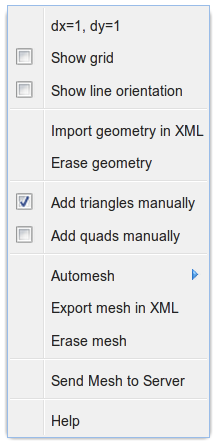
\includegraphics[width=4cm]{me-menu.png}
\end{center}
\vspace{-4mm}
\caption{Mesh Editor's menu.}
\end{figure}


\subsection*{Overview of Menu Functions}

In the order of appearance, the menu functions do the following:
\begin{itemize}
\item Grid spacing: Sets grid spacing in the x and y directions.
\item Show grid: Turns on and off grid display.
\item Show line orientation: By default, each edge is oriented from the older 
node (with a lower index) to the newer one (with higher index). If this checkbox 
is on, edge orientations are shown using arrows. 
\item Import geometry in XML: Imports geometry from a file in XML format.
\item Erase geometry: Discards current geometry.
\item Add triangles manually: If this checkbox is on, ME will suggest triangular
      elements as the mouse is moved over the domain. Left-click to create the element.
\item Add quads manually: If this checkbox is on, ME will suggest quadrilateral
      elements as the mouse is moved over the domain. Left-click to create the element.
\item Automesh: Allows to select a mesh generator (for the time being only 
Triangle is available), define automesh settings, and generate mesh automatically. 
\item Export mesh in XML: Exports mesh in XML format.
\item Erase mesh: Discards current mesh.
\item Send Mesh to Server: Sends mesh to server for further use in calculation.
\item Help: Launches this Help.
\end{itemize}

\subsection*{Importing Geometry in XML}

When ME is launched via the {\tt nclab.mesh\_editor()} command, it does not contain any 
geometry. In that case right-click into the work area and in the menu that appears choose 
Import geometry in XML. Then you can insert a XML geometry file (generated by NCLab’s GE 
or any other software). The format of the XML file is shown at the end of this document.

\subsection*{Manual Mesh Generation}

After a geometry is imported, move the mouse over the domain and ME will suggest triangular 
elements. If this is not the case, please report a bug to {\tt nclab-user@googlegroups.com}. 
If you click on such an element, it is added to the mesh. Double-click will remove it. 
To change the type of elements to quadrilaterals, right-click in the work area and in the 
menu select 

\begin{verbatim}
Add quads manually. 
\end{verbatim}
You can always return back to triangular mode by choosing 

\begin{verbatim}
Add triangles manually. 
\end{verbatim}
Again, double-click removes an element.

\subsection*{Automatic Mesh Generation}

Automatic mesh generation is presently restricted to triangular meshes and 
the only automatic mesh generator supported in NCLab is Triangle. ME 
can handle curved edges.
For automatic mesh generation, select 

\begin{verbatim}
Automesh
\end{verbatim}
in the menu. You will have an opportunity to set the minimum 
angle in the triangulation, as well as maximum triangle area.
Do not generate too large meshes, or the data transfer will 
take lots of time. 
After the mesh is generated, it can be either sent to the server
via the corresponding menu option, or it can be erased and 
you can start over.

\subsection*{XML Mesh Format}

The following mesh file was obtained using the geometry file from the end 
of this document. The Area parameter in subdomains was not set, so only 
nodes contained in the original geometry were used. 

\begin{verbatim}
<mesh_h2d xmlns:xsi="http://www.w3.org/2001/XMLSchema-instance" 
xsi:noNamespaceSchemaLocation="../../include/mesh/mesh_h2d_xml.xsd">
  <vertices>
    <vertex x='0.15' y='-0.049875' id='0'/>
    <vertex x='0.15' y='0.100125' id='1'/>
    <vertex x='-0.15' y='0.100125' id='2'/>
    <vertex x='-0.15' y='-0.049875' id='3'/>
    <vertex x='0' y='-0.049875' id='4'/>
    <vertex x='0' y='0.100125' id='5'/>
  </vertices>
  <elements>
    <triangle v1='3' v2='4' v3='2' marker='Undefined' />
    <triangle v1='2' v2='4' v3='5' marker='Undefined' />
    <triangle v1='5' v2='0' v3='1' marker='Undefined' />
    <triangle v1='0' v2='5' v3='4' marker='Undefined' />
  </elements>
  <boundaries>
    <boundary_edge v1='2' v2='5' marker='top-left'/>
    <boundary_edge v1='4' v2='3' marker='bottom-left'/>
    <boundary_edge v1='4' v2='5' marker='middle-vertical'/>
    <boundary_edge v1='0' v2='4' marker='bottom-right'/>
    <boundary_edge v1='5' v2='1' marker='top-right'/>
  </boundaries>
  <curves>
    <curve v1='2' v2='3' angle='45' marker='left-arc'/>
    <curve v1='1' v2='0' angle='45' marker='right-arc'/>
  </curves>
</mesh_h2d>
\end{verbatim}

\subsection*{XML Geometry Format}

The following is a simple example of a geometry with six nodes, seven edges 
of which two are 45-degree circular arcs, and two subdomains. The <nodes> 
section is self-explanatory, just remember that indices start at 0. In 
the <edges> section, each edge is defined using a pair of node indices, 
an angle and a marker. If the angle is 0, then this is a straight edge, 
otherwise it is a circular arc. In the <subdomains> section, each 
subdomain is defined using a point that is inside, and a marker.

\begin{verbatim}
<geometry>
  <nodes>
    <node x='0.15' y='-0.05' id='0'/>
    <node x='0.15' y='0.1' id='1'/>
    <node x='-0.15' y='0.1' id='2'/>
    <node x='-0.15' y='-0.05' id='3'/>
    <node x='0' y='-0.05' id='4'/>
    <node x='0' y='0.1' id='5'/>
  </nodes>
  <edges>
    <edge start='2' end='5' angle='0' marker='top-left'/>
    <edge start='2' end='3' angle='45' marker='left-arc'/>
    <edge start='4' end='3' angle='0' marker='bottom-left'/>
    <edge start='4' end='5' angle='0' marker='middle-vertical'/>
    <edge start='0' end='4' angle='0' marker='bottom-right'/>
    <edge start='1' end='0' angle='45' marker='right-arc'/>
    <edge start='5' end='1' angle='0' marker='top-right'/>
  </edges>
  <subdomains>
    <subdomain x="-0.075" y="0.025" marker="left"/>
    <subdomain x="0.075" y="0.025" marker="right"/>
  </subdomains>
</geometry>
\end{verbatim}


\subsection*{Known Bugs}

No known bugs at this time. Please report bugs to {\tt nclab-user@googlegroups.com}.
\end{document}

